% !TEX root = ../main.tex

% = = = = = = = = = = = = = = = = = = = = = = = = = = = = = = = = = = = = = = = = = = = = = = %
%
%
%
%
%
%
% = = = = = = = = = = = = = = = = = = = = = = = = = = = = = = = = = = = = = = = = = = = = = = %

\section{Threat Model}

The attack surface to abuse users' browsers through cryptojacking is broad, and there are multiple vectors where various entities can inject mining scripts in the website's codebase. We summarize those here. 

\subsection{Webmaster initiated} 

A website administrator can add a mining script to her webpage, with or without informing users. Website owners may do this to monetize their sites, especially when they have been blacklisted or blocked by standard advertising platforms. In one example, a researcher found Coinhive on a large Russian website offering child pornography to users~\cite{coinhiveonchildporn}. Revenue estimates, based on the website traffic data available, were roughly \$10,000 a month after converting the value of XMR mined to USD.

\subsection{Mixed content} 

Many websites serve active Javascript from third parties within their own webpages. This could be ads from an ad network or tools for tracing users of their site. Third parties with these privileges can inject cryptojacking scripts into the sites that use them. For example, Showtime claims this is how CoinHive was deployed within their site~\cite{showtimehive}. In two separate incidents, Coinhive was injected into the websites of Movistar\footnote{Movistar is a major telecommunications brand owned by Telefonica, operating in Spain and in many Hispanic American countries \url{https://www.movistar.com/}} and Globovision\footnote{Globovision is a 24-hour television news network in Venezuela and Latin America.\url{http://globovision.com/}} using Google Tag Manager.\footnote{Google Tag Manager is a tag management system created by Google to manage JavaScript and HTML tags used for tracking and analytics on websites} Movistar stated that Coinhive was not put on their website by a hacker, but instead was due to \textit{``internal error''} while they were conducting ``production tests.'' No statement was provided by Globovision on why the cryptojacking scripts appeared on their site on November 15, 2017~\cite{googletagcoinhive}.

\subsection{Browser extensions} 

Cryptojacking was not limited to websites in 2017. The chrome extension Archive Poster remained on the Chrome Web Store for days while silently cryptojacking an unknown portion of their 100,000+ users. After multiple user reports, followed by multiple news media outlets covering the issue, the extension was removed~\cite{chromeextentioncoinhive}. 

\subsection{Breaches} 

If an attackers is able to breach principle websites, extensions, or the scripting services they use, they can inject cryptojacking scripts that will impact the site's users without the site's knowledge or consent. For example, a researcher found a malicious modification to webchat system LiveHelpNow's SDK; it resulted in unsolicited mining across all websites using their char support service~\cite{chatsupporthack}. In another example, Coinhive was found on the political fact-checking website Politifact.\footnote{PolitiFact: Fact-checking US politics.\url{https://politifact.com/}} A compromised JavaScript library was found to be injecting the cryptojacking scripts. The malicious code remained on the site for at least four hours before it was removed~\cite{politifactcoinhive}. PolitiFact Executive Director stated ``Hackers were able to install their script on the fact-checking website after discovering a misconfigured cloud-computing server''~\cite{politifactcoinhivewsj}.


\subsection{Man-in-the-middle} 

A user's webtraffic is often routed through intermediaries that may have plaintext access to content. For example, internet service providers or free public wireless routers can inject cryptojacking scripts into non-HTTPS traffic. Advertisement code injection has been seen in practice ~\cite{vergeadinjection}. There have been assertions of similar injections of browser mining scripts at certain Starbucks free Wi-Fi hotspots.\footnote{\url{https://twitter.com/imnoah/status/936948776119537665}}






% = = = = = = = = = = = = = = = = = = = = = = = = = = = = = = = = = = = = = = = = = = = = = = %
%
%
%
%
%
%
% = = = = = = = = = = = = = = = = = = = = = = = = = = = = = = = = = = = = = = = = = = = = = = %

\section{Measurements}

\subsection{Prevalence of Coinhive and alternatives}

\begin{figure}[t]
\centering
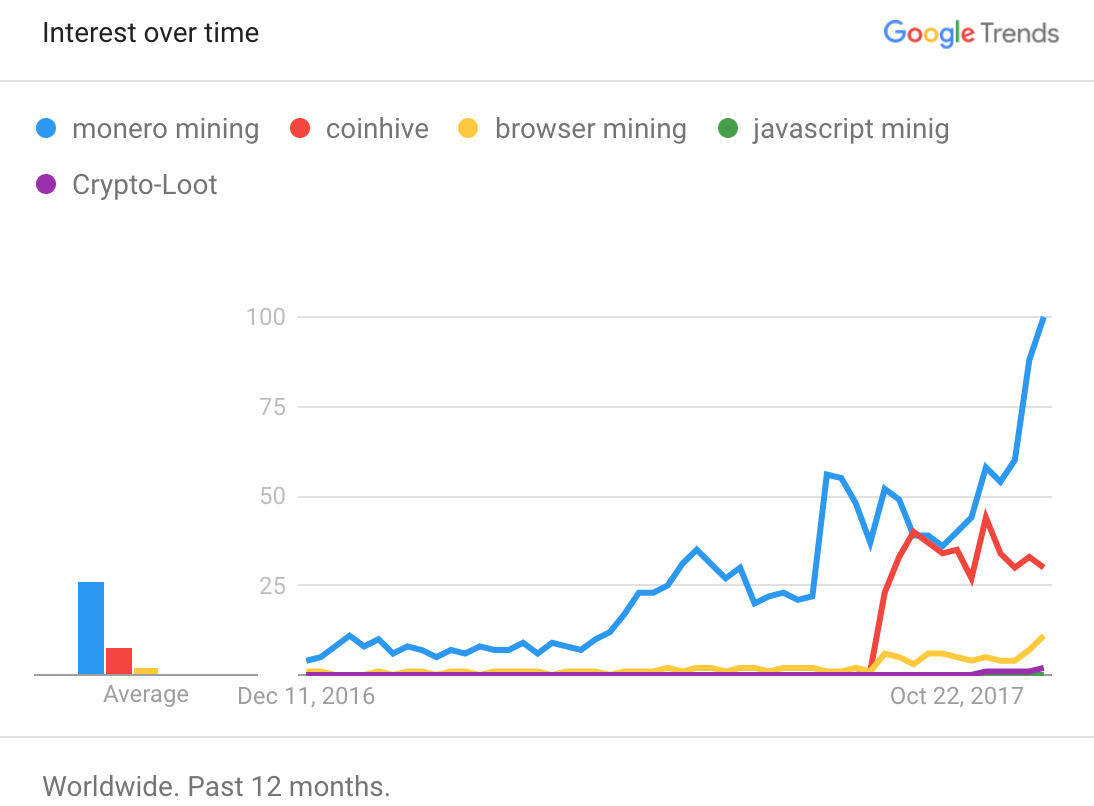
\includegraphics[width=0.9\linewidth]{figures/usage_over_time2.png}
\caption{Google Trend over last 12 months: there has been more interest in Coinhive than the broader, related search term ``Browser mining''. Comparing to other services offering Monero browser mining API, Coinhive had the advantage of being the first to offer the service. \label{fig:trend}}
\end{figure}

\begin{figure}[t]
\begin{tabular}{c}
\begin{lstlisting}[language=sql]
SELECT domain, tags, p80.http_www.get.headers.content_language, p80.http_www.get.headers.server, p80.http.get.headers.x_powered_by, p80.http.get.title, p80.http_www.get.body as wwwbody, p80.http.get.body as plainbody 
FROM censys-io.domain_public.20171123
WHERE STRPOS(p80.http.get.body, coinhive.min.js) > 0 or STRPOS(p80.http_www.get.body, coinhive.min.js) >0)
\end{lstlisting}
\end{tabular}
\caption{A BigQuery SQL query to find websites that embed the CoinHive script using a dataset of the top one million sites from censys.io. \label{lst:bigquery}}
\end{figure}

\begin{figure}[t]
\centering
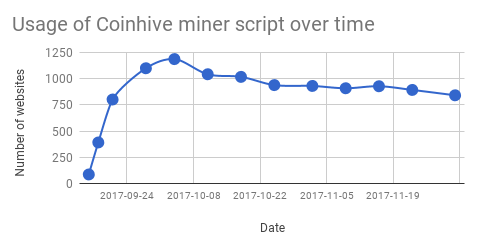
\includegraphics[width=\linewidth]{figures/usage_of_coinhive_over_time.png}
\caption{The number of instances of the Coinhive miner scripts found using the query in Figure~\ref{lst:bigquery} in top one million websites over a three month period beginning with the release of Coinhive in September 2017.\label{fig:topmil}}
\end{figure}

We focus on measuring the prevalence of Coinhive scripts deployed on internet sites. We use the censys.io BigQuery dataset ~\cite{censys15} for the top million sites indexed by Zmap.\footnote{\url{https://zmap.io}} We simply look for the \texttt{coinhive.min.js} script within the body of the website page. The query we use is in Figure~\ref{lst:bigquery} and the results over a two month period are provided in Figure~\ref{fig:topmil}. These findings are corroborated by another search engine, PublicWWW, which indexes the source code of publicly available websites. Using PublicWWW's dataset, over 30,000 websites were found to have the \texttt{coinhive.min.js} library~\cite{badpacketspublicwww}. As seen from our data in Figure~\ref{fig:topmil}, the adoption of this script was substantial in the first days of its release. However, progress slowed down at the same time as ad-blockers and organizations started to block Coinhive's website. The initial purpose of this service, as claimed by Coinhive, was to replace ads and cover server costs for webmasters. As the service did not require that website's received user consent before beginning to mine, it started to be used maliciously in user's browsers. This type of usage resulted in Coinhive being included in some company's top-10 most wanted malware list~\cite{checkpoint}.

This type of measurement will become less accurate moving forward. Cryptojacking services are evolving to use obfuscated JavaScript and randomized URLs to evade detection\footnote{\url{https://twitter.com/bad_packets/status/940333744035999744}}. An example of these methods can be found in the cryptojacking service provider called Minr. In this case, the script is automatically obfuscated for users implementing the code. In addition, the domain names used by Minr frequently change to circumvent blocklists and anti-malware software.

\begin{figure}[t]
\centering
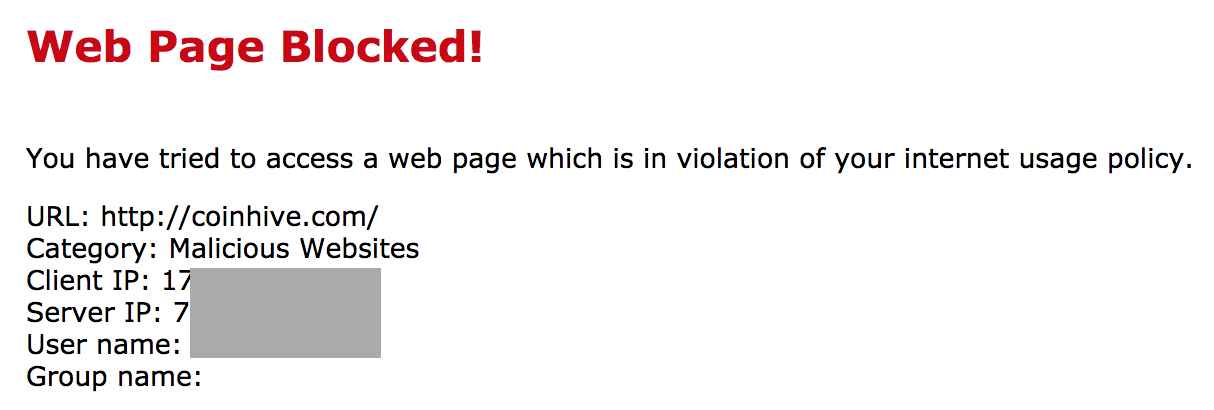
\includegraphics[width=0.9\linewidth]{figures/coinhive_blocked.png}
\caption{Our university has categorized the coinhive.com website as malicious and has blocked it.\label{fig:concordia}}
\end{figure}

\begin{figure}[t]
\centering
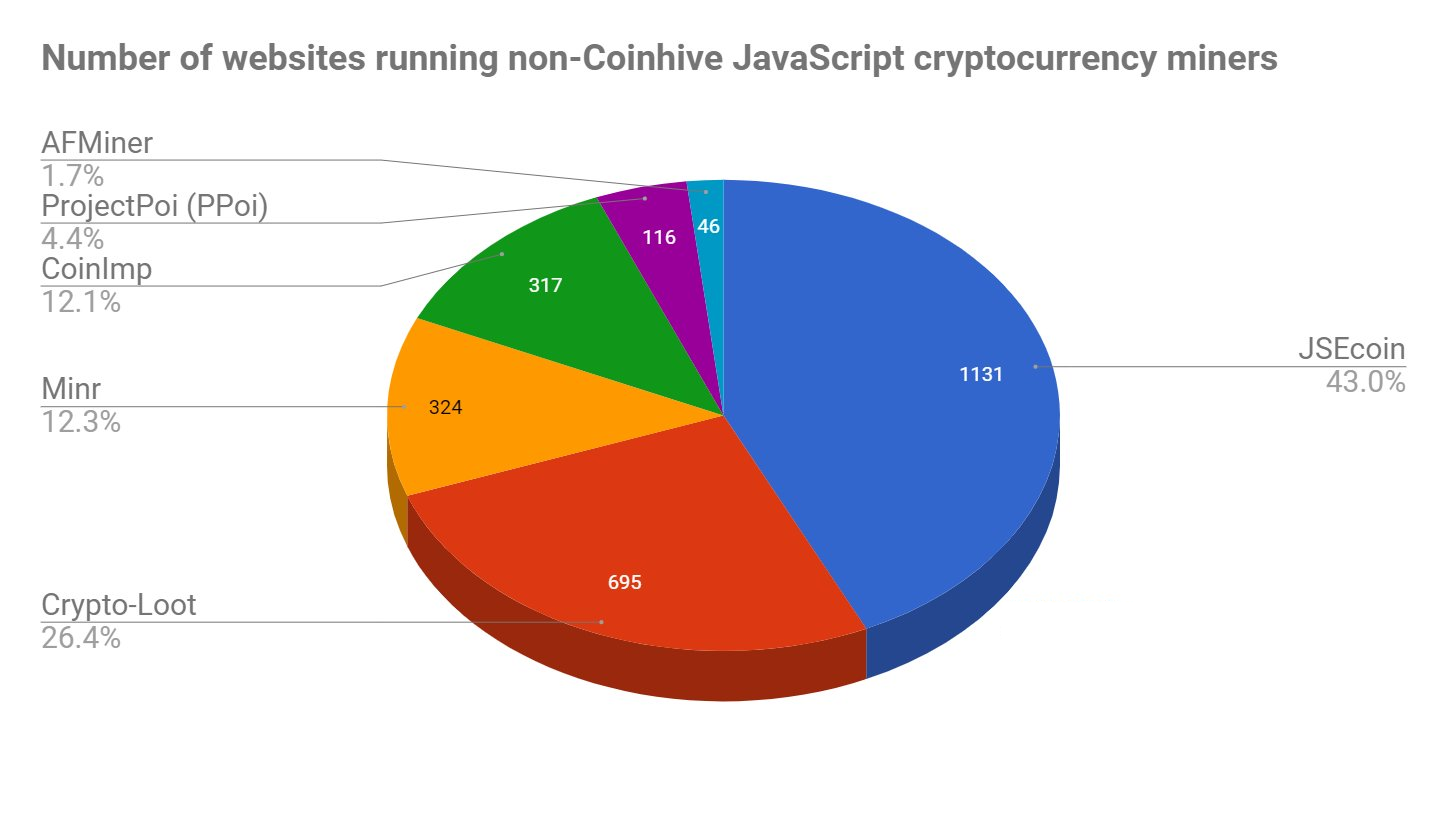
\includegraphics[width=0.9\linewidth]{figures/non-coinhive-miners.png}
\caption{Share of websites using a Coinhive alternative as gathered from PublicWWW~\cite{badpacketspublicwww}.\label{fig:copycat}}
\end{figure}

Coinhive has begun to be blocked by enterprises. One example is shown in Figure~\ref{fig:concordia}. This blocking seems to have sent Coinhive operators to lesser known alternatives with the same or similar functionality (see Figure~\ref{fig:copycats}). Coinhive has also reacted by focusing on adding user consent and legitimizing the use of cryptojacking.




\subsection{Clientside Impact}

\begin{figure}[t]
\centering
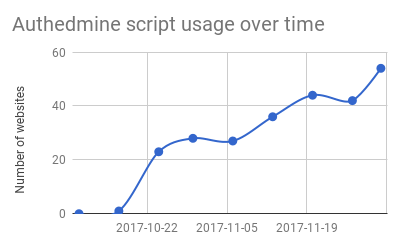
\includegraphics[width=0.9\linewidth]{figures/usage_of_authedmine_over_time.png}
	\caption{Usage of AuthedMine Miner scripts in top 1million websites over time.}
\end{figure}

Coinhive introduced another domain and service called ``Authedmine'' , which requires user`s consent to start mining in the browser. This service did not get the same attention as the original service, but it did inspire discussions regarding the ethics of such services, which is covered in Discussion section of this paper. (Clickjacking) 

Most of these scripts discovered were configured to use around 25\% of user`s CPU, which can be justified as it will be under the threshold of attracting the user`s attention, and it could be argued as fair-usage of their hardware. During the first few days, however, there were some reports of 100\% CPU usage when visiting websites containing these scripts~\cite{piratesbayblog}, which can be characterized as malicious. By default, the Coinhive JavaScript library will use all available CPU resources available. The user implementing the script must include a throttle value to reduce the client-side CPU usage during mining operations.

\begin{figure}[t]
\centering
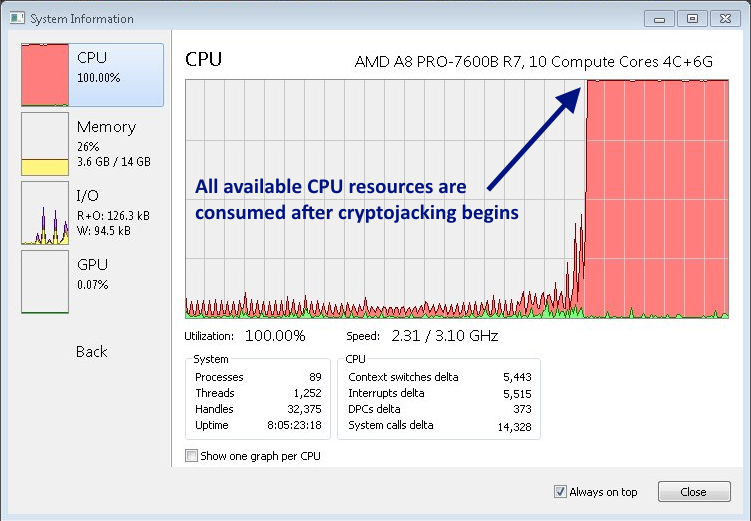
\includegraphics[width=\linewidth]{figures/windows_cpu_usage.png}
	\caption{Comparison of CPU usage of browser without and with browser mining enabled}
\end{figure}

\subsection{Profitability}
\label{profitabilitexperiment}

Coinhive developers estimate a monthly revenue of about 0.3 XMR (~\$101) for a website with 10-20 active miners, which would be users with longer duration of visit on the website~\cite{coinhive}.

Through correspondence with one of the biggest coinhive campaigns operator, which was a domain parking service and was running coinhive script on over 11,000 parked websites, conducted over period of three months, we were able to gather some data to estimate profitability for websites with high traffic but short visits \footnote{Collaborated with Faraz Fallahi \url{https://github.com/fffaraz}}. Over 97,000 users visited these websites for an average of 24 seconds per session.


\begin{figure}[t]
\centering
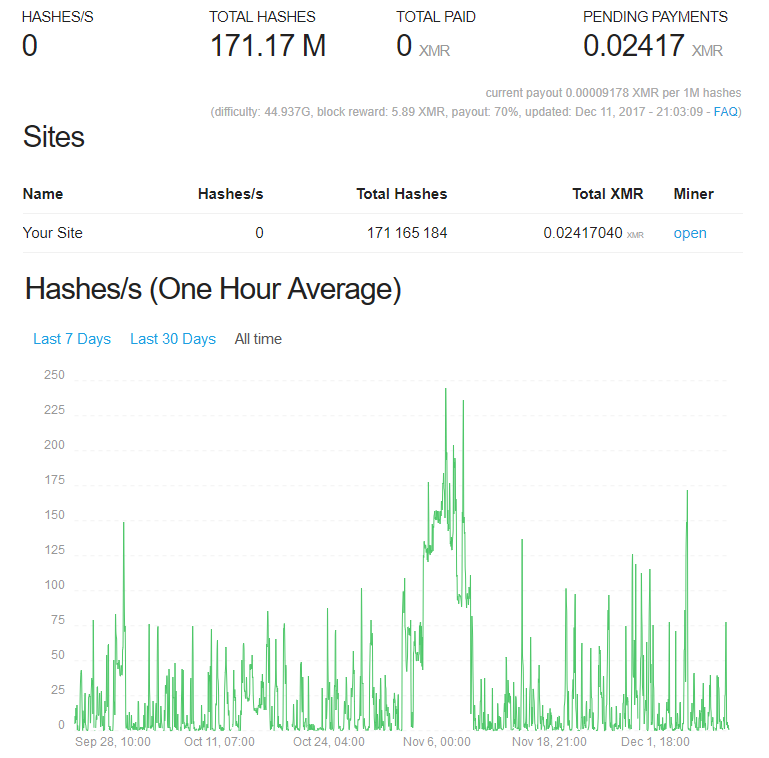
\includegraphics[width=\linewidth]{figures/experiment_coinhive_results.png}
\caption{Coinhive dashboard showing the earnings over the course of 3 months}
\end{figure}



%TODO: THIS CAN BE REMOVED AS WE TALK ABOUT THE NUMBERS IN THE TEXT
\begin{figure}[t]
\centering
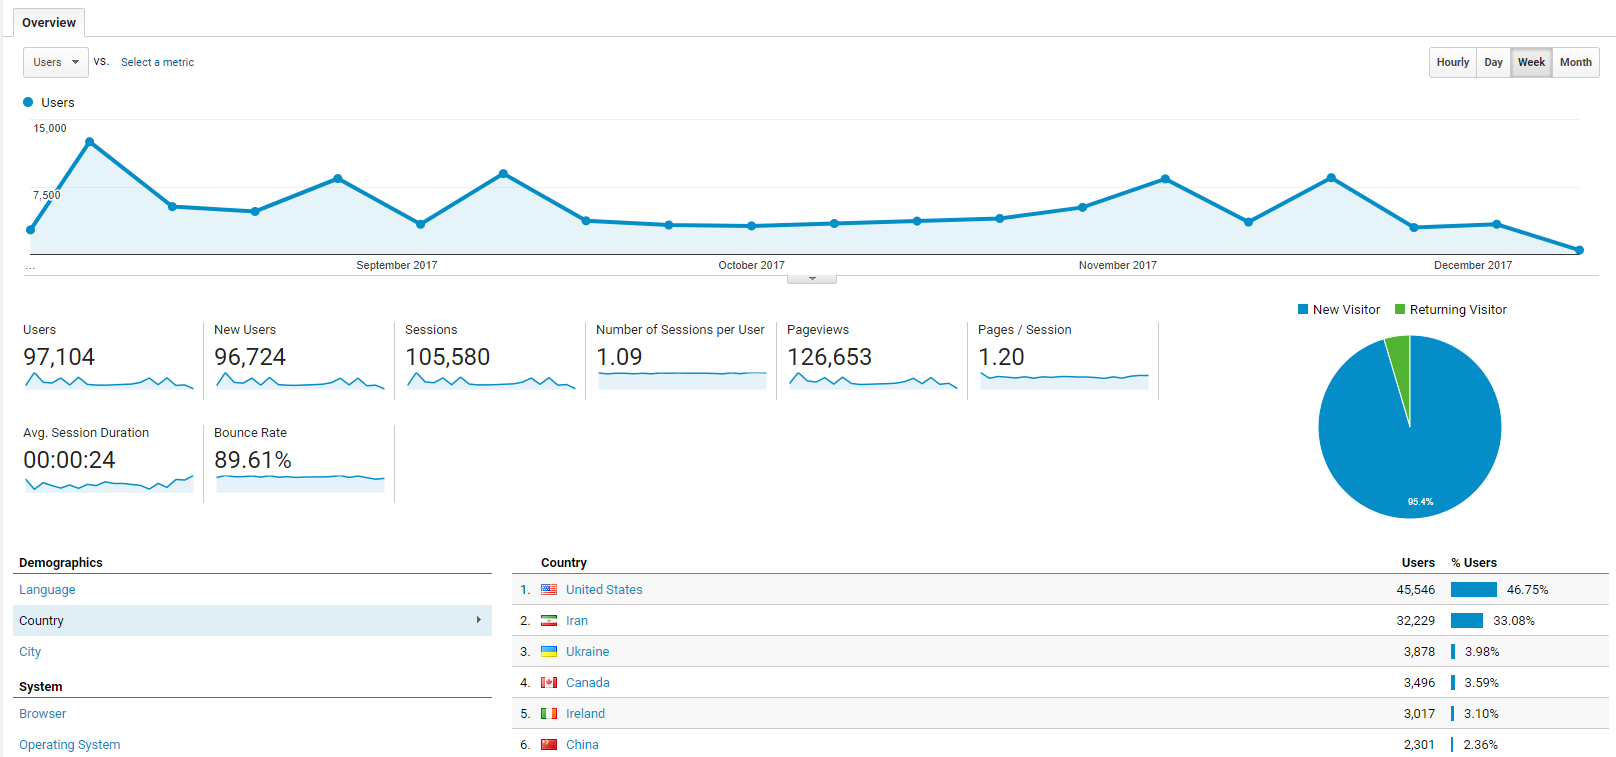
\includegraphics[width=\linewidth]{figures/experiment_analytics_results.png}
\caption{Google Analytics dashboard}
\end{figure}


This experiment showed that even though the number of users visiting was significant, the profit from those visits was below expectations. For the period examined, the revenue was 0.02417 Monero, which at the time of writing is equivalent to 7.69 USD.


% = = = = = = = = = = = = = = = = = = = = = = = = = = = = = = = = = = = = = = = = = = = = = = %


\section{Ethical Considerations}

The opinion of the authors of this paper maintain that users should be given the option to enable the miner code in their browser only with some benefit to their experience on the website. Recent polls support this notion, such as the one conducted by Bleeping Computer, which found that ``many users said they are OK with websites mining Monero in the background if they don`t see ads anymore''~\cite{bleepingcomputerminers}. Another example would be granting access to premium features of the website such as journal articles behind a paywall, or streaming in high-definition. The website could also allow the user to participate in mining rewards by allocating a large portion of their CPU resources to the activity of mining, which would benefit both parties. By notifying the user of the potentials of such activity, and allowing them to make a choice to participate, the website maintains trust in their relationship with the user while also benefiting from a new source of revenue. By foregoing disclaiming this new activity, which can have harmful effects, the website will gain a new revenue stream for a short time only while sacrificing their reputation in the long term. Coinhive`s recent response to the market`s negative reaction by releasing AuthedMine, which enforces user consent before enabling any mining JavaScript code, justifies this rationale. However, before consented browser mining could develop into a sustainable model, its security implications and user impact should be addressed.

Browser developers are starting to talk about throttling or blocking such scripts\footnote{Please consider intervention for high cpu usage js \url{https://bugs.chromium.org/p/chromium/issues/detail?id=766068}}  ~\cite{operanocoin}, however this discussion need further considerations as throttling should happen based on some variables, in which might affect legitimate applications as well. Also if they switch to user notification for high CPU usage per website, the notification itself might not be affective as desired~\cite{SHB11}\cite{SEAAC09}.

Coinhive as a big player in the recent rise of in-browser mining, introduced its functionality as a replacement for online advertisement, a new way to monetize website`s traffic. However this will result in a paradigm shift in website monetization. As an example in both auction-based and keyword-based online advertisement, the advertiser pays the ad publisher to distribute the ads and the ad publisher pays a portion of the revenues to the website owner whom the ad was shown on her website~\cite{king2007internet}. However in in-browser mining as a replacement monetization strategy, user is technically paying for their website visit on their hydro (electricity) bill, in which the consent of the user becomes an ethical issue. 

As the concept of website traffic revenue begins to change, the values associated with the old concept will have to be reexamined. Moor, in "What is Computer Ethics?" ~\cite{moor1985computer} introduces the concept of \textit{Invisible Factor}, for invisible computer operations in society. Based on his definitions cryptojacking falls under \textit{Invisible abuse}, the intentional use of the invisible operations of a computer to engage in unethical conduct. Here the cryptojacker is earning money from unaware users that are being charged on their hydro bill. 

%TODO: this paragraph can be shortened. the point is the story of piratesbay and how they dealth with it
Most browser mining code is ran without the consent, nor knowledge, of the users involved. As previously mentioned, the websites that have been found running JavaScript code for the purpose of mining usually employed Coinhive`s API. One such website, for example, ThePirateBay.org~\cite{bbcmintcrypto}, which ran the JavaScript code when users searched for torrent files. Perhaps unsurprisingly, there was no notice in their Privacy Policy nor visible warning on any part of the website that informed their users of this activity. This resulted in a backlash against the website, which responded with the following statement, ``Do you want ads or do you want to give away a few of your CPU cycles every time you visit the site?'' ~\cite{piratesbayblog}. While they admitted to their testing of browser mining, their notice came after the fact and resulted in the removal of the JavaScript code altogether due to upset users. This is in contrast to the banners users are presented with upon the first visit to a website that warns them of the website`s policy on cookies, which is enforced today through EU laws~\cite{eucookie}. It is now widely known that these cookies can be used to track users across the internet, so cookie banners can act as a reminder and allow the user to make better informed decisions regarding their browsing habits. Without any type of disclaimer for users, websites have been commandeering their users` CPU resources for their business and personal gain. This results in higher energy bills for the user, along with accelerated device degradation, slower system performance, and poor web experience~\cite{httparchiveminingimpact}\cite{gaurdianelectricity}.


%TODO: the next two paraphraphs also has been talked about before. can combine both together.
A second example of a popular website deploying Coinhive`s API is Showtime.com, which is a popular cable channel that also streams their TV shows online. Showtime has declined to comment on how or why Coinhive was implemented on their website. Speculation has been raised that it was injected via an third-party analytics tool, New Relic, due to Coinhive being found inside the New Relic code block within website's source code. However a New Relic representative denied these claims in a statement to The Register, "It appears they [Coinhive scripts] were added to the website by its [Showtime's] developers." ~\cite{registershowtime}. 
It was then hardly surprising when UFC.com was accused of using this very same code on the night of streaming one of their most popular events~\cite{registerufcmonero}. In a statement released by the UFC, they denied the presence of the code stating, ``[they] did not find any reference to the mentioned Coinhive JavaScript [code]``\footnote{\url{https://twitter.com/bad_packets/status/928044219222048769}}.
 
The recent trend of streaming websites deploying Coinhive's API could be due to the high costs of providing streaming services. While ads can be used to offset some of those costs, it would be of interest to some to at least experiment with the idea of recruiting their users to mine Monero for profit. This same regard is true for hackers looking to maximize their cryptojacking profits. The longer a user is engaged on a website, such as video streaming service, the more income can be earned through browser mining.

Given the recent interest some websites have shown in regard to browser mining, there is also potential for this new form of revenue generation to compete with advertisements. As seen in section~\ref{profitabilitexperiment}, an immediate impact could be to reduce how many ads a user sees on a given website. Moving forward websites with long user sessions such as streaming services could one day even replace ads. This is because the malware that is associated with advertisements is still a growing concern, and the public`s dislike of advertisements will likely persist and not wane. Also, as cryptocurrencies continue to grow in market capitalization and use cases, their inevitable mainstream use will push the profitability of mining egalitarian proof-of-work cryptocurrencies, such as Monero, well into the future. 

%The lack of regulation in cryptocurrency space allows for a grey market to grow. This is felt more when it affects non-tech-savvy users. 


% = = = = = = = = = = = = = = = = = = = = = = = = = = = = = = = = = = = = = = = = = = = = = = %

\section{Mitigations}

One possible solution is to enforce user consent on service provider level. One example for this is that Coinhive started Authedmine to enforce user consent before running the miners, Although Clickjacking~\cite{rydstedt2010busting} and other methods of obfuscation has been used to bypass this enforcement model and run the miner code without the proper authorization.

Similar to regulations for cookies and user tracking there is a need to regulate browser mining, primarily to notify users of the existence of these scripts on the webpages they visit. Also, there is a need to standardize this model, so to answer some of these questions: If every website uses a browser miner and users have many tabs open, how are CPU resources shared between them? How will the behaviour of these scripts change based on the device they are running on? If device is on power saving mode, how will that affect the execution of these scripts?

In addition to regulation and standardizing, better security design is required to narrow down the attack surface, such as using SSL/TLS and tokenizing the requests to make sure websites get user`s consent before running these scripts. DNS TXT records could also be implemented to verify domain name ownership before browser mining scripts would be authorized to run on the website.

Surveys with larger sample size and diversity is required to gauge users acceptance. These surveys should answer how much CPU power users are willing to volunteer, and if battery impact would change their affinity for participation.

Browser mining has been shown to not be as efficient as native mining applications today. Therefore, optimizations on how browsers pass system calls to the operating system can be made, or there can even be browsers designed specifically to support efficient browser mining. However, browsers such as Opera, have taken a stance against cryptojacking scripts and blocked them via "NoCoin" blacklist ~\cite{operanocoin}. The effectiveness of using a blacklist to block such activities is still not clear. %maybe a bit more on this? meaning that as seen so far, cryptojackers can just use new domains/ips to bypass these blacklists

This new model of monetizing websites can be a paradigm shift in how advertisement giants monopolize internet traffic. This could lead to re-democratizing the online advertisement ecosystem to make it fairer for smaller players.

% = = = = = = = = = = = = = = = = = = = = = = = = = = = = = = = = = = = = = = = = = = = = = = %

\section{Concluding Remarks}



















